\documentclass{beamer}
\usepackage[utf8]{inputenc}
\usepackage{hyperref}

\usetheme{Madrid}
\usecolortheme{beaver}
\hypersetup{colorlinks=true, linkcolor=blue, filecolor=magenta, urlcolor=cyan}
\urlstyle{same}

\title{Amateur Telescope Making}
\subtitle{...or how to make your own telescope at home}
\author{Nuno Miguel Sousa}
\institute{Coimbra, Portugal}
\date{\today}

\begin{document}

\begin{frame}
\titlepage
\end{frame}

\begin{frame}
\frametitle{What is Amateur Telescope Making?}
\begin{block}{}
Amateur Telescope Making, or ATM, is a hobby taken by people that have an interest in astronomic observation and enjoy building telescopes.\footnotemark
\end{block}
\footnotetext{\url{https://en.wikipedia.org/wiki/Amateur_telescope_making}}
\begin{block}{}
ATM can range from just assembling the individually bought components to actually fabricate some or all of the components of a telescope.
\end{block}
\begin{block}{}
The most common type of telescope made by hobbyists is the so called Newtonian reflector (invented by Sir Isaac Newton).\footnotemark
\end{block}
\footnotetext{\url{https://en.wikipedia.org/wiki/Newtonian_telescope}}
\end{frame}

%\begin{frame}
%\frametitle{Why build a telescope?}
%\begin{itemize}
%\item Have a better understanding of how telescopes are built and how they work.
%\item Knowing the 
%\item Just for fun?
%\end{itemize}
%\end{frame}

\begin{frame}
\frametitle{My personal motivation for ATM}
\begin{columns}
\column{0.6\textwidth}
One time by chance a few years ago, I had the opportunity to look up at the night sky in Alentejo's countryside, in southern Portugal.

The combination of very low light pollution and clear sky provided for a very distinctive view of the Milky Way.

I had some interest in astronomy in general, but that event was what sparked the beggining of my interest in astronomical observation and ended up in deciding to build a telescope myself.
\column{0.4\textwidth}
\begin{figure}
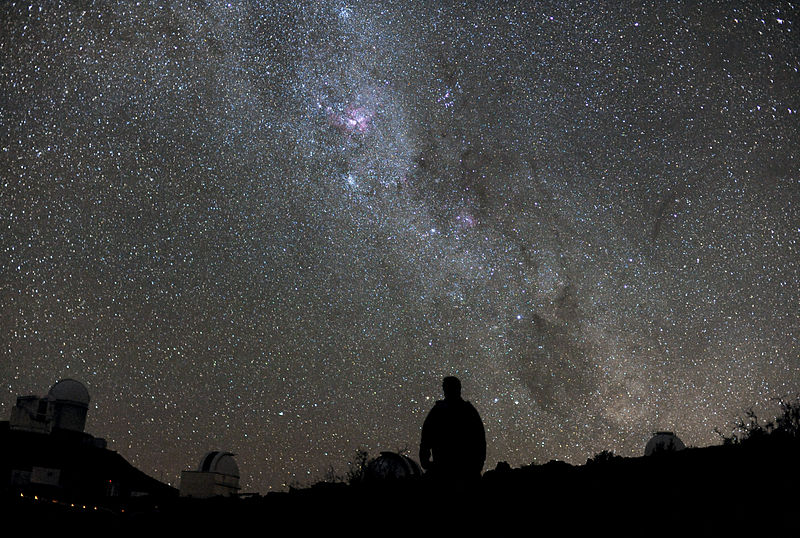
\includegraphics[scale=0.45]{assets/800px-Starry_Night_at_La_Silla.jpg}
\caption{Not me!}
\end{figure}
\end{columns}
\end{frame}

\begin{frame}
\frametitle{What I'm building.}
My name is Nuno and ...
\end{frame}

\begin{frame}
\frametitle{About the author}
My name is Nuno and ...
\end{frame}

\begin{frame}
\frametitle{The end}
Thank you!
\end{frame}

\end{document}
